% Chapter Template

\chapter{Models} % Main chapter title

\label{ch:models} % Change X to a consecutive number; for referencing this chapter elsewhere, use \ref{ChapterX}

\lhead{Chapter 2. \emph{Models}} % Change X to a consecutive number; this is for the header on each page - perhaps a shortened title

%----------------------------------------------------------------------------------------
%	SECTION: INTRO
%----------------------------------------------------------------------------------------

\section{Introduction to Models}
In this section we present the models used in demonstrating the uncertainty quantification (UQ) methods in this
work.  We use the term \emph{model} to describe any code with uncertain inputs and a set of at least one
response quantity of interest.  Because the efficiency of polynomial chaos expansion methods is strongly dependent on the continuity
of the response, we demonstrate a variety of models with varying levels of continuity.

We include a variety of models with the intent to demonstrate the strengths and weaknesses of each UQ
method.

Firstly, we include several analytic models.  These are models who have an exact, derivable value for
statistical moments or sensitivities.  They are simpler in mechanics than full engineering-scale problems, and
offer a way to benchmark the performance of the UQ methods.

Secondly, we include an engineering-scale multiphysics application.  There are no analytic response values in
this model, only a nominal case with no uncertainty included in the input space.  Demonstration of the
performance of UQ methods on this model will highlight the practical application of each method.

We describe each model in turn.  Throughout the models, we will describe them using the syntax
\begin{equation}
  u(Y) = Q,
\end{equation}
where $u(Y)$ is the model as a function of $N$ uncertain inputs $Y=(y_1,\ldots,y_N)$ and $Q$ is a
single-valued response quantity of interest.  $Q$ may also be a vector of single-valued quantities of interest and the methods
described apply equally well; for our purposes, we only consider single-valued responses.

Another factor that impacts the performance of polynomial chaos expansion methods is the dimensionality of the input space.  Despite 
many methods to curtail the curse of dimensionality described in Chapter \ref{Chapter3}, collocation for polynomial chaos expansion
is fundamentally a grid-based method.  Because of this, the efficiency of polynomial chaos methods will degrade quickly as
dimension increases.  To demonstrate how the efficiency of the various methods we use in this work, we select models that are
easily extensible to multiple dimensions and high-order polynomials.  As a result, most of the models are tensor products of
polynomials.

%----------------------------------------------------------------------------------------
%	SECTION: TENSOR POLY
%----------------------------------------------------------------------------------------

\section{Tensor Monomials}\label{mod:first tensor poly}
The simplest model we make use of is a first-order tensor polynomial (tensor monomial) combination \ref{Ayres}.
Each term in this polynomial expression is at most linear in any dimension.  This provides a simple calculation
of the statistical moments, and no second-order polynomials are required to exactly reproduce this model.
The mathematical expression for tensor monomials is
\begin{equation}
  u(Y) = \prod_{n=1}^N (y_n+1).
\end{equation}
For example, for $N=3$ we have
\begin{equation}
  u(Y) = y_1y_2y_3 + y_1y_2 + y_1y_3 + y_2y_3 + y_1 + y_2 + y_3 + 1.
\end{equation}
For this model we distribute the uncertain inputs in several ways because of its simplicity: uniformly on [-1,1], uniformly on
[0,1], and normally on [$\mu,\sigma$]. A summary of analytic statistics is given in Table \ref{tab:tensormono moments}.
The two-dimensional representation of this function is given in Figure \ref{fig: tensor monomials}.
\begin{figure}[htb]
  \centering
  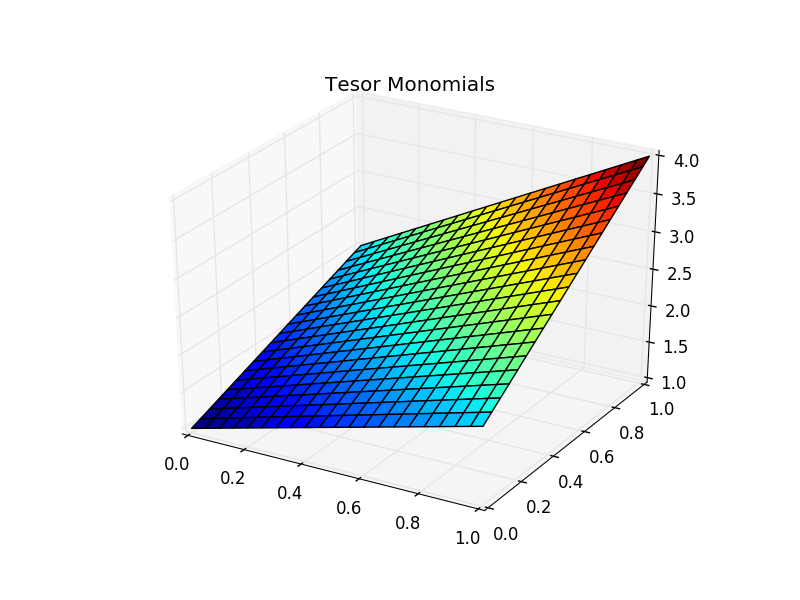
\includegraphics[width=0.7\linewidth]{anlmodels/tensor_monom}
  \caption{Tensor Monomials}
  \label{fig: tensor monomials}
\end{figure}

\begin{table}[H]
  \centering
  \begin{tabular}{c|c|c}
    Distribution & Mean & Variance \\\hline
    $\mathcal{U}[-1,1]$ & 1 & $\qty(\frac{4}{3})^N - 1$ \\
    $\mathcal{U}[0,1]$ & $\qty(\frac{3}{4})^N$ & $\qty(\frac{7}{3})^N - \qty(\frac{3}{4})^{2N}$ \\
    $\mathcal{N}[\mu,\sigma]$ & $\prod_{n=1}^N (\mu_{y_n}+1)$ & $\prod_{n=1}^N[(\mu_{y_n}+1)^2+\sigma_{y_n}^2]
    - \prod_{n=1}^N (\mu_{y_n}+1)^2$
  \end{tabular}
  \caption{Analytic Expressions for Tensor Monomial Case}
  \label{tab:tensormono moments}
\end{table}
For purposes of demonstration, we pick several increasing orders of dimensionality: three input variables, five variables, and 
ten variables.

%----------------------------------------------------------------------------------------
%	SECTION: Sudret
%----------------------------------------------------------------------------------------
\section{Sudret Polynomial}\label{mod:sudret}
The polynomial used by Sudret in his work \cite{sudret} is another tensor-like polynomial, and is a test case traditionally used to
identify convergence on sensitivity parameters.  It is similar to tensor monomials because it is constructed by the tensor
product of simple polynomials; in this case, Sudret used second-order polynomials.  As a result, only zeroth or second-order
polynomials exist in the expression.  Statistical moments are also quite straightforward for this model.
The mathematical expression for Sudret polynomials is
\begin{equation}
  u(Y) = \frac{1}{2^N}\prod_{n=1}^N (3y_n^2+1).
\end{equation}
The two-dimensional representation of this function is given in Figure \ref{fig: sudret}.
\begin{figure}[htb]
  \centering
  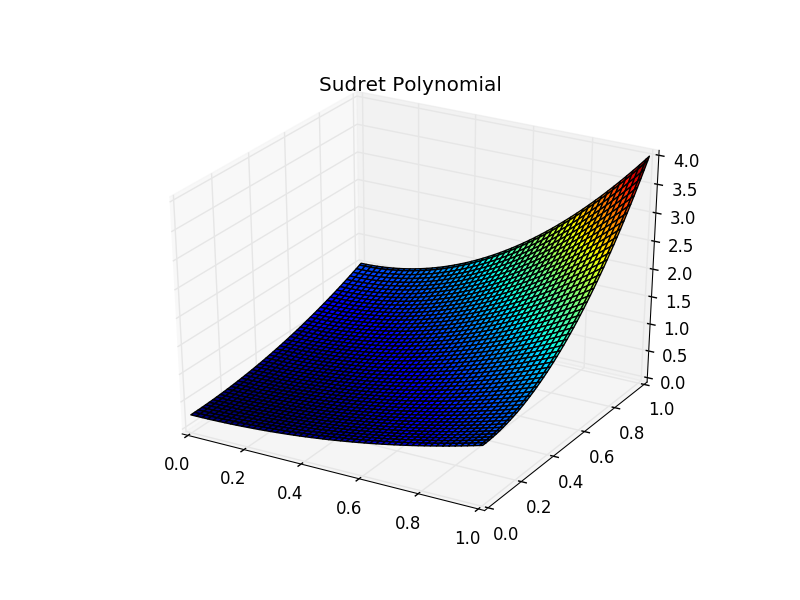
\includegraphics[width=0.7\linewidth]{anlmodels/sudret}
  \caption{Sudret Polynomial}
  \label{fig: sudret}
\end{figure}
The variables are distributed uniformly on [0,1].

The statistical moments and sensitivities are given in
Table \ref{tab:sudret}, where $\mathcal{S}_n$ is the global Sobol sensitivity of $u(Y)$ to perturbations in
$y_n$.

\begin{table}[H]
  \centering
  \begin{tabular}{c c}
    Statistic & Expression \\\hline
    Mean & 1 \\
    Variance & $\qty(\frac{6}{5})^N - 1$ \\
    $\mathcal{S}_n$ & $\frac{5^{-n}}{(6/5)^N-1}$
  \end{tabular}
  \caption{Analytic Expressions for Sudret Case}
  \label{tab:sudret}
\end{table}
Because of its similarity to tensor polynomials, the cases we show are three inputs and five inputs.

%----------------------------------------------------------------------------------------
%	SECTION: ATTENUATION
%----------------------------------------------------------------------------------------
\section{Attenuation}\label{mod:attenuation}
While this model is also a tensor product and analytic, it also is the solution to a physical problem.
Consider a one-dimensional problem that consists of a material with unit length and vacuum to the left and
right of the material.  We consider a beam of neutral particles that have a probability of interacting
with the material, or passing through it.  This beam enters the material on the left and exits on the right.
The quantity of interest is the percent of particles that pass through the material without interacting
anywhere along its length.  The boundary conditions for this problem are a constant flux on the left boundary,
and a vacuum boundary on the right boundary.

This model represents an idealized single-dimension system where an beam of particles impinges on a
purely-absorbing material with total scaled length of 1.  The response of interest is the fraction of
particles exiting the opposite side of the material.  The material is divided into $N$ segments, each of which
has a distinct uncertain absorption cross section $y_n$.  The solution takes the form
\begin{equation}
  u(Y) = \prod_{n=1}^N \exp(-y_n/N).
\end{equation}
The two-dimensional representation of this function is given in Figure \ref{fig: attenuation}.
\begin{figure}[htb]
  \centering
  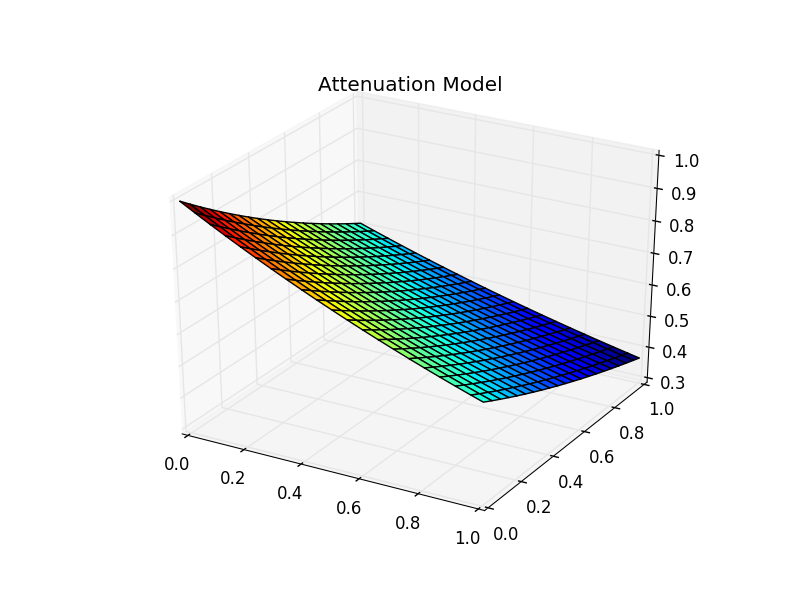
\includegraphics[width=0.7\linewidth]{anlmodels/attenuate}
  \caption{Attenuation Model}
  \label{fig: attenuation}
\end{figure}
Because negative cross sections have dubious physical meaning, we restrict the distribution cases to uniform
on [0,1] as well as normally-distributed on [$\mu,\sigma$].  A summary of analytic statistics is given in
Table \ref{tab:attenuation moments}.

\begin{table}[H]
  \centering
  \begin{tabular}{c|c|c}
    Distribution & Mean & Variance \\\hline
    $\mathcal{U}[0,1]$ & $\qty[N\qty(1-e^{-1/N})]^N$ & $\qty[\frac{N}{2}\qty(1-e^{-2/N})]^N -
                       \qty[N\qty(1-e^{-1/N})]^{2N}$ \\
    $\mathcal{N}[\mu,\sigma]$ & $\prod_{n=1}^N \exp\qty[\frac{\sigma_{y_n}^2}{2N^2}-\frac{\mu_{y_n}}{N}]$
    & $\prod_{n=1}^N \exp\qty[\frac{2\sigma_{y_n}^2}{N^2} - \frac{2\mu_{y_n}}{N}]$
  \end{tabular}
  \caption{Analytic Expressions for Attenuation Case}
  \label{tab:attenuation moments}
\end{table}

This model has some interesting properties to demonstrate performance of polynomial-based UQ methods.  First,
because the solution is a product of exponential functions, it cannot be exactly represented by a finite
number of polynomials.  Second, the Taylor development of the exponential function includes all increasing
polynomial orders.  The product of several exponential functions is effectively a tensor combination of
polynomials for each dimension.

%----------------------------------------------------------------------------------------
%	SECTION: Gaussian Peak
%----------------------------------------------------------------------------------------
\section{Gaussian Peak}\label{mod:gausspeak}
Similar to the attenuation model, the Gaussian peak \cite{sfugenz} instead uses square arguments to the
exponential function.  A tuning parameter $a$ can be used to change the peakedness of the
function.  Increased peakedness leads to more difficult polynomial representation.  
A location parameter $\mu$ can be used to change the location of the peak.
The mathematical expression is
\begin{equation}
  u(Y) = \exp\qty(-\sum_{n=1}^N a^2\qty(y_n-\mu)^2).
\end{equation}
We allow each $y_n$ to vary uniformly on [0,1].
The two-dimensional representation of this function is given in Figure \ref{fig: gauss peak}.
\begin{figure}[htb]
  \centering
  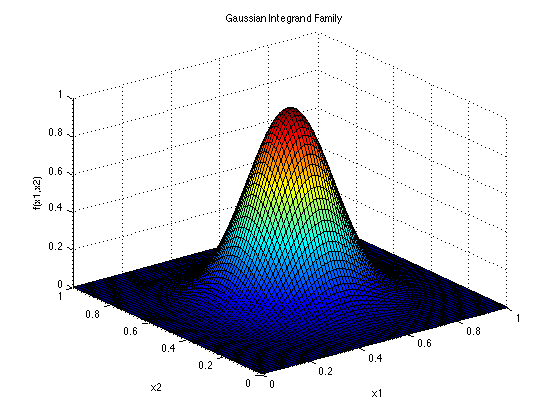
\includegraphics[width=0.7\linewidth]{anlmodels/gaussian}
  \caption{Gaussian Peak \cite{sfu}}
  \label{fig: gauss peak}
\end{figure}
A summary of analytic statistics is given in Table \ref{tab:gausspeak moments}.

\begin{table}[H]
  \centering
  \begin{tabular}{c|c}
    Statistic & Expression \\ \hline
    Mean & $\qty(\frac{\sqrt{\pi}}{2a}\qty(\erf(a\mu)+\erf(a-a\mu)))^N$ \\
    Variance & $\qty(\frac{\sqrt{\pi/2}}{2a}\qty(\erf(a\mu\sqrt{2})-\erf(a\sqrt{2}(1-\mu))))^N - \qty(\frac{\sqrt{\pi}}{2a}\qty(\erf(a\mu)+\erf(a-a\mu)))^{2N}$
  \end{tabular}
  \caption{Analytic Expressions for Gaussian Peak Case}
  \label{tab:gausspeak moments}
\end{table}
This case offers particular challenge because of its Taylor development, which only includes even powers of
the uncertain parameters.  This suggests added difficulty in successive representation, especially for an
adaptive algorithm.


%----------------------------------------------------------------------------------------
%	SECTION: Ishigami
%----------------------------------------------------------------------------------------
\section{Ishigami Function}\label{mod:ishigami}
The Ishigami function \cite{ishigami} is a commonly-used function in performing sensitivity analysis.  It is
given by
\begin{equation}
  u(Y) = \sin{y_1} + a\sin^2{y_2} + b y_3^4\sin(y_1).
\end{equation}
In our case, we will use $a=7$ and $b=0.1$ as in \cite{ishigami2}. 
The graphical representation of this function is given in Figure \ref{fig: ishigami}, with the three axes
as the three inputs and the color map as the function values ranging approximately from -10.74 to 17.74.
\begin{figure}[htb]
  \centering
  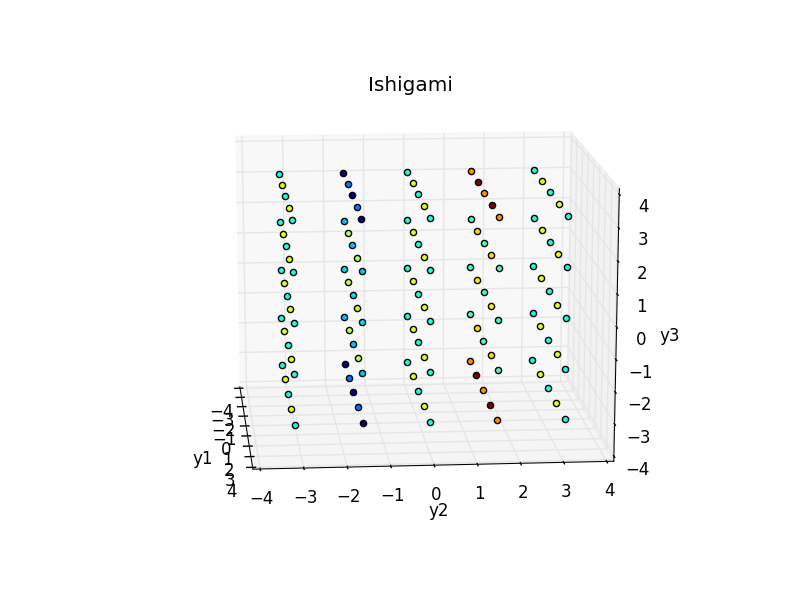
\includegraphics[width=0.7\linewidth]{anlmodels/ishigami}
  \caption{Ishigami Model}
  \label{fig: ishigami}
\end{figure}
In particular interest for this model are
its strong nonlinearity and lack of independence for $y_3$, as it only appears in conjunction with $y_1$.  The
analytic statistics of interest for this model are in Table \ref{tab:ishigami moments}, where $D_n$ is the
partial variance contributed by $y_n$ and Sobol sensitivities $\mathcal{S}_n$ are obtained by dividing $D_n$
by the total variance.

\begin{table}[H]
  \centering
  \begin{tabular}{c|c|c}
  Statistic & Expression & Approx. Value \\\hline
  Mean & $\frac{7}{2}$ & 3.5 \\
  Variance & $\frac{a^2}{8} + \frac{b\pi^4}{5} + \frac{b^2\pi^8}{18} + \frac{1}{2}$ & 13.84459 \\
  $D_1$ & $\frac{b\pi^4}{5} + \frac{b^2\pi^8}{50} + \frac{1}{2} $ &  4.34589 \\
  $D_2$ & $\frac{a^2}{8}$ & 6.125 \\
  $D_{1,3}$ & $\frac{8b^2\pi^8}{225}$ & 3.3737 \\
  $D_3,D_{1,2},D_{2,3},D_{1,2,3}$ & 0 & 0
  \end{tabular}
  \caption{Analytic Expressions for Ishigami Case}
  \label{tab:ishigami moments}
\end{table}


%----------------------------------------------------------------------------------------
%	SECTION: Sobol G-Function
%----------------------------------------------------------------------------------------
\section{Sobol G-Function}\label{mod:gfunc}
The so-called ``g-function'' introduced by Saltelli and Sobol \cite{gfunc} is a discontinuous 
function used most commonly as a test for sensitivity coefficients.  The function is often used as an integrand 
for numerical estimation methods \cite{gfuncM}.  
The function is given by
\begin{equation}
  u(Y) = \prod_{n=1}^N \frac{\abs{4y_n-2}-a_n}{1+a_n},
\end{equation}
where
\begin{equation}
  a_n = \frac{n-2}{2}.
\end{equation}
The two-dimensional representation of this function is given in Figure \ref{fig: g func}.
\begin{figure}[htb]
  \centering
  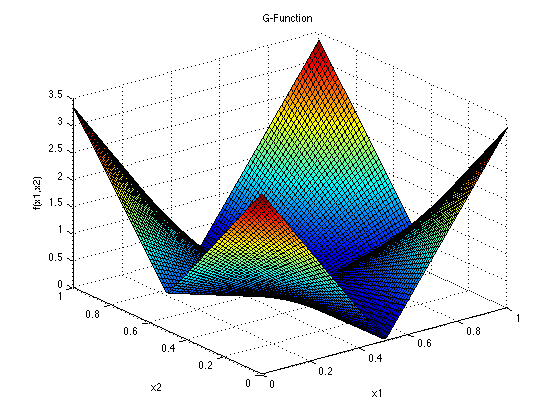
\includegraphics[width=0.7\linewidth]{anlmodels/gfunc}
  \caption{Sobol G-Function \cite{sfu}}
  \label{fig: g func}
\end{figure}


There are some implementations \cite{gfuncM} that force $a_n \geq 0$, which allows for a simple
understanding of the sensitivity coefficients: 
\begin{itemize}
  \item $a_n=0$: $y_n$ is very important
  \item $a_n=1$: $y_n$ is relatively important,
  \item $a_n=9$: $y_n$ is non-important,
  \item $a_n=99$: $y_n$ is non-significant.
\end{itemize}
However, for our purposes, we set no limit to the value of $a_n$, as our interest is primarily in the moments
instead of the sensitivity coefficients.

We select this model because it offers the challenge of a function
without a continuous first derivative.  We expect the polynomial representations to perform poorly
in this instance, and more so as dimensionality increases.
%----------------------------------------------------------------------------------------
%	SECTION: Anisotropic
%----------------------------------------------------------------------------------------
\section{OECD Benchmark}
TODO move from time-dep chapter to here?

\section{Pin Cell}\label{mod:pincell}
TODO move this to mammoth results chapter?

This model is a coupled multiphysics engineering-scale model.  It simulates fuel behavior through the depletion of fissile material
in a single two-dimensional slice of a fuel rod.  The problem domain contains the fuel, gap, clad, and
moderator, and represents a symmetric quarter pin.  The depletion steps are carried out through a year-long
burn cycle.
The coupled multiphysics are neutronics, handled by \rattlesnake{}, and fuel performance, handled by
\bison{}.  

The mesh is shown in Fig. \ref{fig:pincell mesh}.  TODO BETTER FIGURE.  The mesh contains 20 bands of fuel
blocks, the gap, the clad, and the moderator.  TODO Use colors to describe locations.  TODO dimensions.
\begin{figure}[htb]
  \centering
  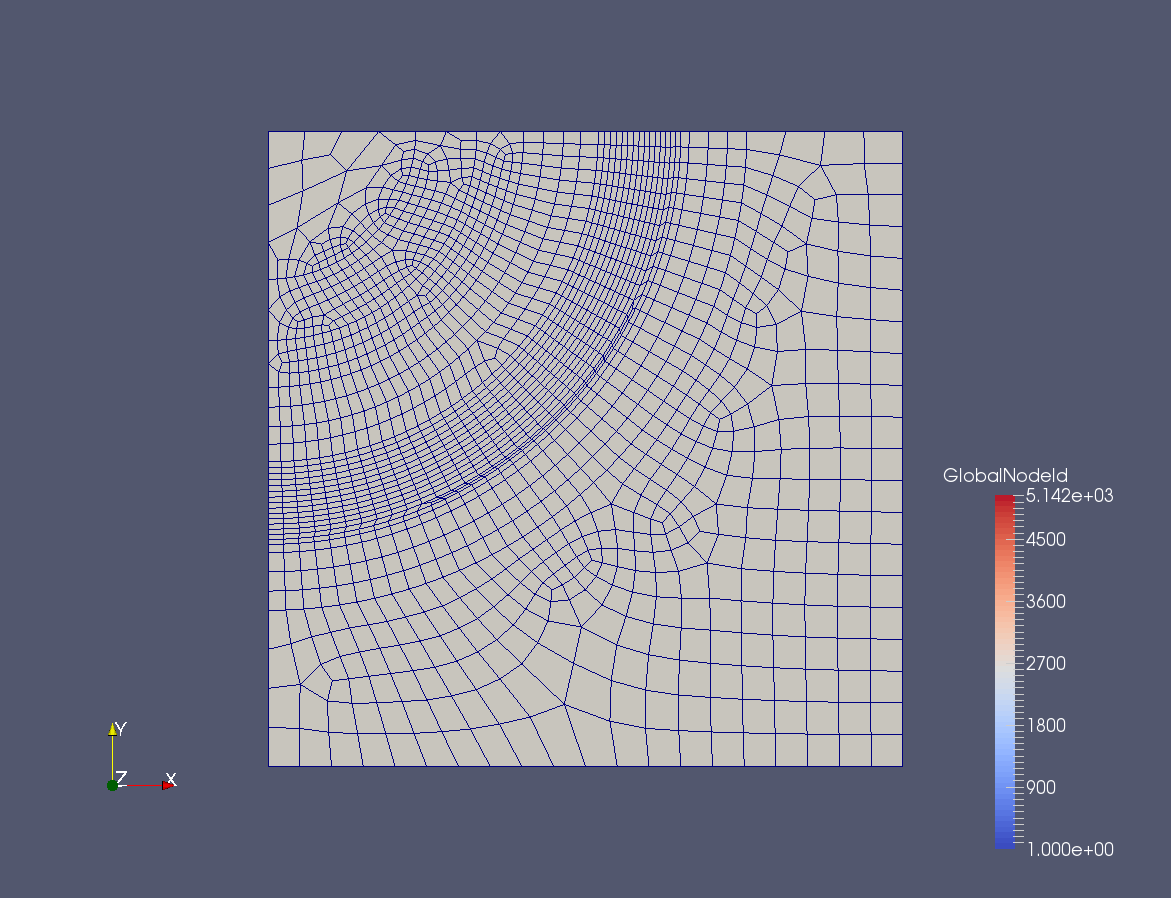
\includegraphics[width=0.7\linewidth]{pincell_mesh_png}
\end{figure}

The neutronics is calculated using 8 energy groups and takes as uncertain inputs 671 material cross
sections, including fission, capture, scattering, and neutron multiplication factor  Each cross section is
perturbed by 10\% of its original value, distributed normally.  The scattering cross
sections for each material in each group are not perturbed individually; rather, a scattering scaling factor
for each group is determined, and the scattering cross sections are all scaled by that factor.  The fission
and capture cross sections are perturbed individually.  The critical output of the neutronics calculation is
power shapes for use in the fuel performance code, as well as the $k$-eigenvalue for the rod.

The fuel performance code models mechanics such as heat conduction in the fuel, clad, and gap, clad stresses, grain radius
growth, and fuel expansion through the depletion steps of the fuel. The code takes power shapes
from the neutronics code as input and produces several key characteristics, such as peak clad temperature, maximum
fuel centerline temperature, and maximum clad stress.

The uncertain input space is highly correlated, so a Karhunen-Loeve (KL) component analysis is performed as
the first step in a two-part reduction \cite{physor2016}. The
covariance matrix is obtained via cross section construction in \texttt{scale}\cite{scale} using random sampling.  
Table \ref{tab:pcarank} gives the first several eigenvalues in the KL expansion.  Surrogate (or
\emph{latent}) dimensions identified by the KL expansion will be used as input variables for demonstration of
the various UQ methods.

TODO update this for importanceRank

\begin{table}[H]
  \centering
  \begin{tabular}{c|c}
Index & Eigenvalue \\ \hline
1 & 0.974489839965 \\
2 & 0.0183147250746 \\
3 & 0.00271597405394 \\
4 & 0.00260939137165 \\
5 & 0.000486257522596 \\
6 & 0.000431957645049 \\
7 & 0.000253683187786 \\
8 & 0.000228044411204 \\
9 & 0.000124030638175 \\
10 & 7.14328494102e-05 \\
11 & 6.30833696364e-05 \\
12 & 3.87071149672e-05 \\
13 & 3.51066363934e-05 \\
14 & 2.48699823434e-05 \\
15 & 1.98915286765e-05 \\
16 & 1.35985387253e-05 \\
17 & 1.128896325e-05 \\
18 & 9.59426898684e-06 \\
19 & 8.11612567548e-06 \\
20 & 7.16508951777e-06 \\
21 & 6.53366817241e-06 \\
22 & 4.50006575957e-06 \\
23 & 4.19287192651e-06 \\
24 & 3.7671309151e-06 \\
25 & 2.61683536224e-06 \\
26 & 2.22099981728e-06 \\
27 & 1.6360971709e-06 \\
28 & 1.13245742809e-06 \\
29 & 9.92282537141e-07
\end{tabular}
\caption{KL Expansion Eigenvalues for Pin Cell Problem}
\label{tab:pcarank}
\end{table}
